\documentclass[12pt]{article}
\usepackage{graphicx}


\begin{document}

\title{Beam XY-Position at the Target for CLAS/EG6} 
\author{S. Stepanyan and N. Baltzell}
\date{\today}
\maketitle

\section{Introduction}

CLAS tracking algorithm reconstructs track parameters at the production vertex by extrapolating the fitted track in the CLAS drift chambers to the plane perpendicular to mid-plane of each CLAS sector. It takes interception point as a production vertex. This sector dependent plane, ($X^\prime Z^\prime$) where $Z^\prime$ is the direction of the beam and coincides with CLAS $Z$, gets rotated for each sector. For example, for sector 1 ($X^\prime Z^\prime$) plane is the same as CLAS nominal ($YZ$) plane, for sector 4 it is ($-YZ$), while for sector 2 $X^\prime$ is rotated by $-60$ degree relative to the CLAS $X$. After extrapolation of the track to the ($X^\prime Z^\prime$) plane vertex coordinates are transformed to the CLAS coordinate system taking $Z=Z^\prime$, $X$ and $Y$ get calculated using sector rotations. It is assumed always that beam is at ($0.,0.$) point in ($X,Y$) plane. Of course the correct procedure would have been to extrapolate the track to the closest point to the beam and take that point as a production vertex (for detached vertexes things will be different). 

The downside of the current algorithm for reconstruction of the vertex parameters is that ($XY$) vertex coordinates of the track do not carry any real information (see Fig.\ref{fig:xytrack}), although they still can be used for example to cut out outliers. This way of vertex determination works at some level when no magnetic field is present outside of the drift chamber regions, namely around the target. (Although closer look to ($XY$) vertex reconstruction reveals that swimming to ($X^\prime Z^\prime$) plane also has minor error, as shown in Fig.\ref{fig:xytrackc}. This is most likely due to the step size of 0.5 mm that amkes vertex planes shifted from $Y^\prime =0$ plane.) 
\begin{figure}[htb]
\begin{center}
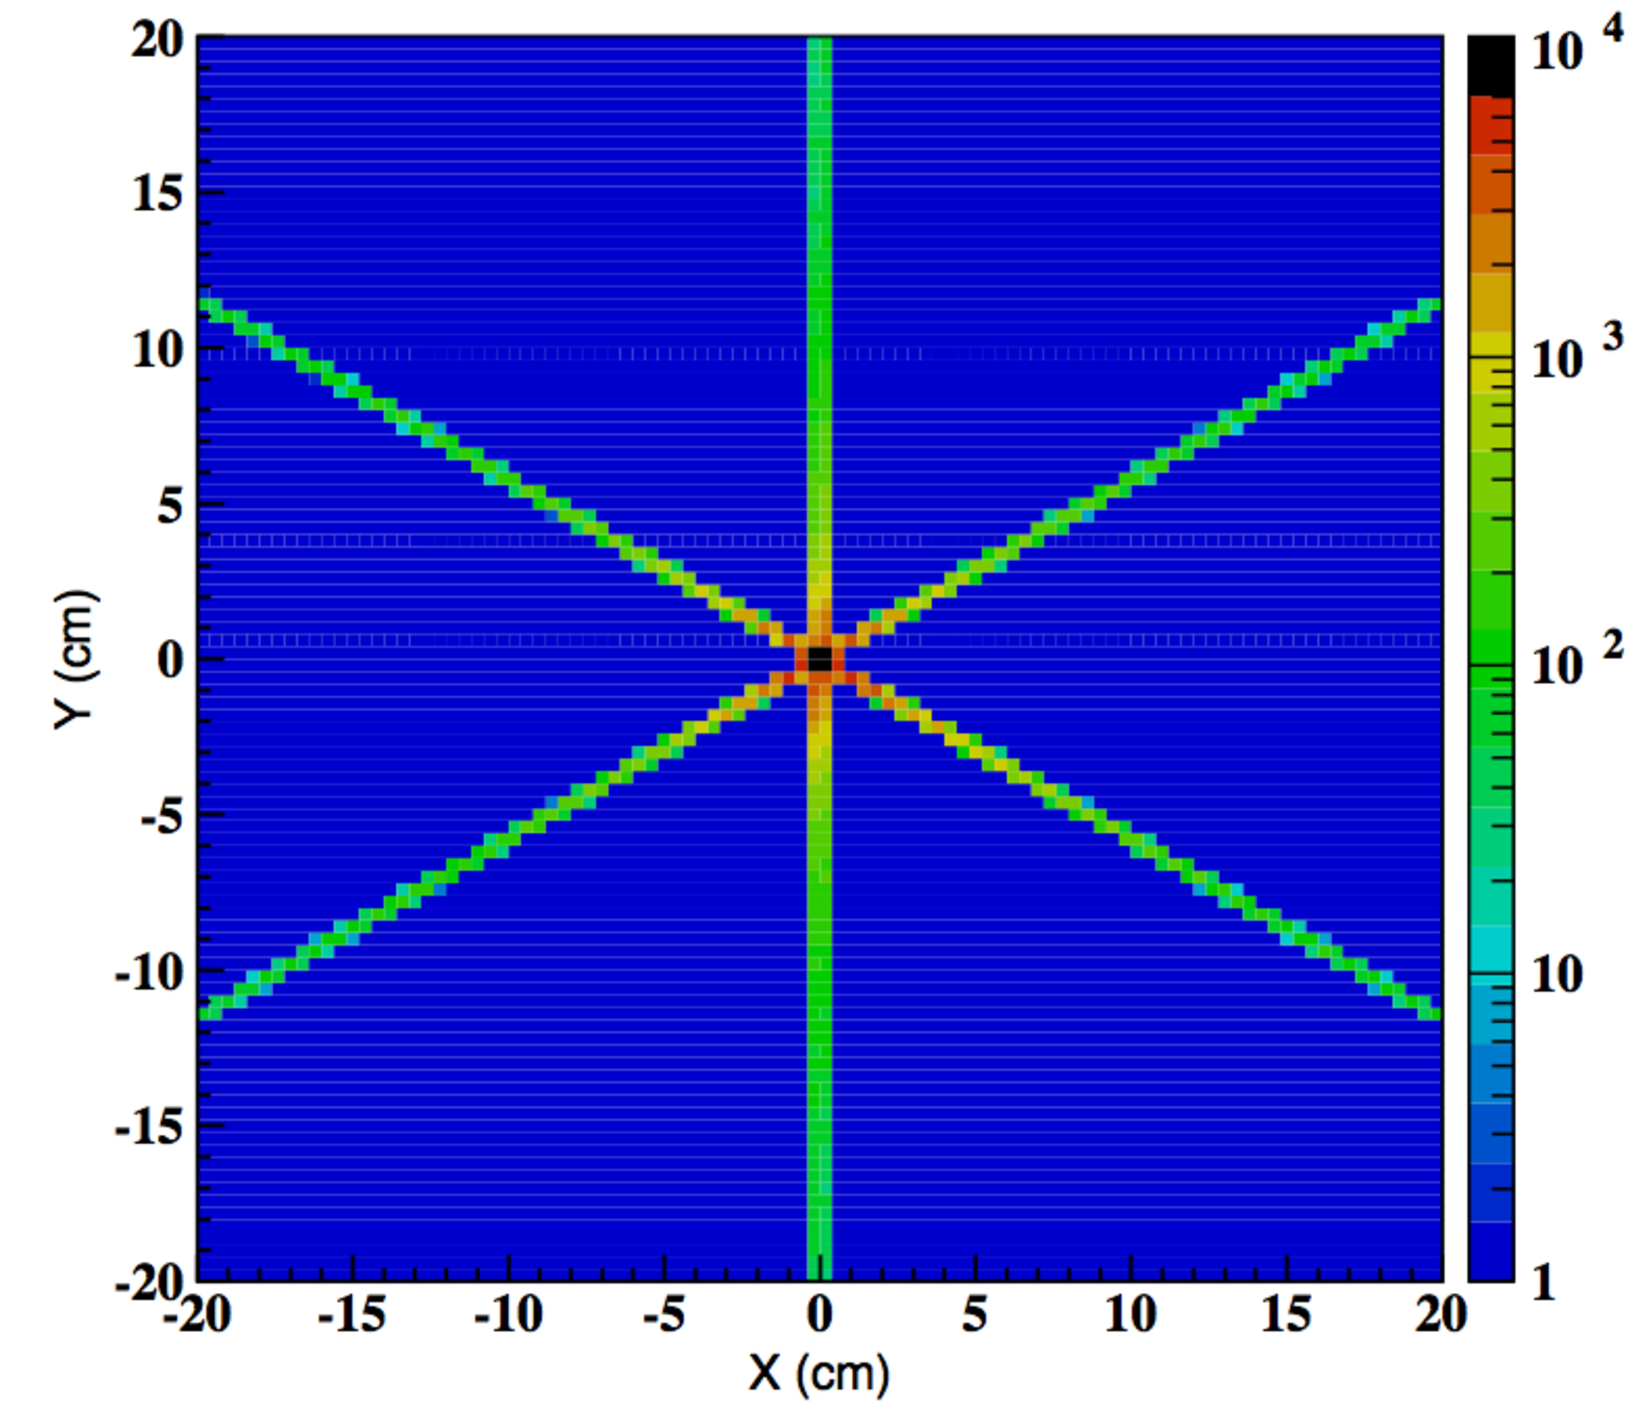
\includegraphics[width=0.75\textwidth]{track_xy}
\caption{Vertex ($XY$) coordinate for charged tracks in CLAS.}
\label{fig:xytrack}
\end{center}
\end{figure}

Incorrect vertex determination effects only vertex coordinate if there is no magnetic field around the target. Track's direction vector is not effected by where the track vector is terminated. Things get complicated when magnetic field is present. In the presence of a field, incorrect fitting to the true production vertex will result in an incorrect determination of the track direction vector. Set of experiments in CLAS used strong (4-5 T) longitudinal solenoid field around the target. In this case vertex parameters of tracks were reconstructed after swimming the track through the field region to the empirical ($X'Z'$) plane. Clearly, if the true production vertex is far from the extrapolation point, e.g. beam does not go through $X=0$ and $Y=0$ point, then the azimuthal angle $\phi$ of the track will be reconstructed incorrectly. Value of the $\phi$ kick will depend on the magnitude of the transverse momentum and the field value. 

\begin{figure}[htb]
\begin{center}
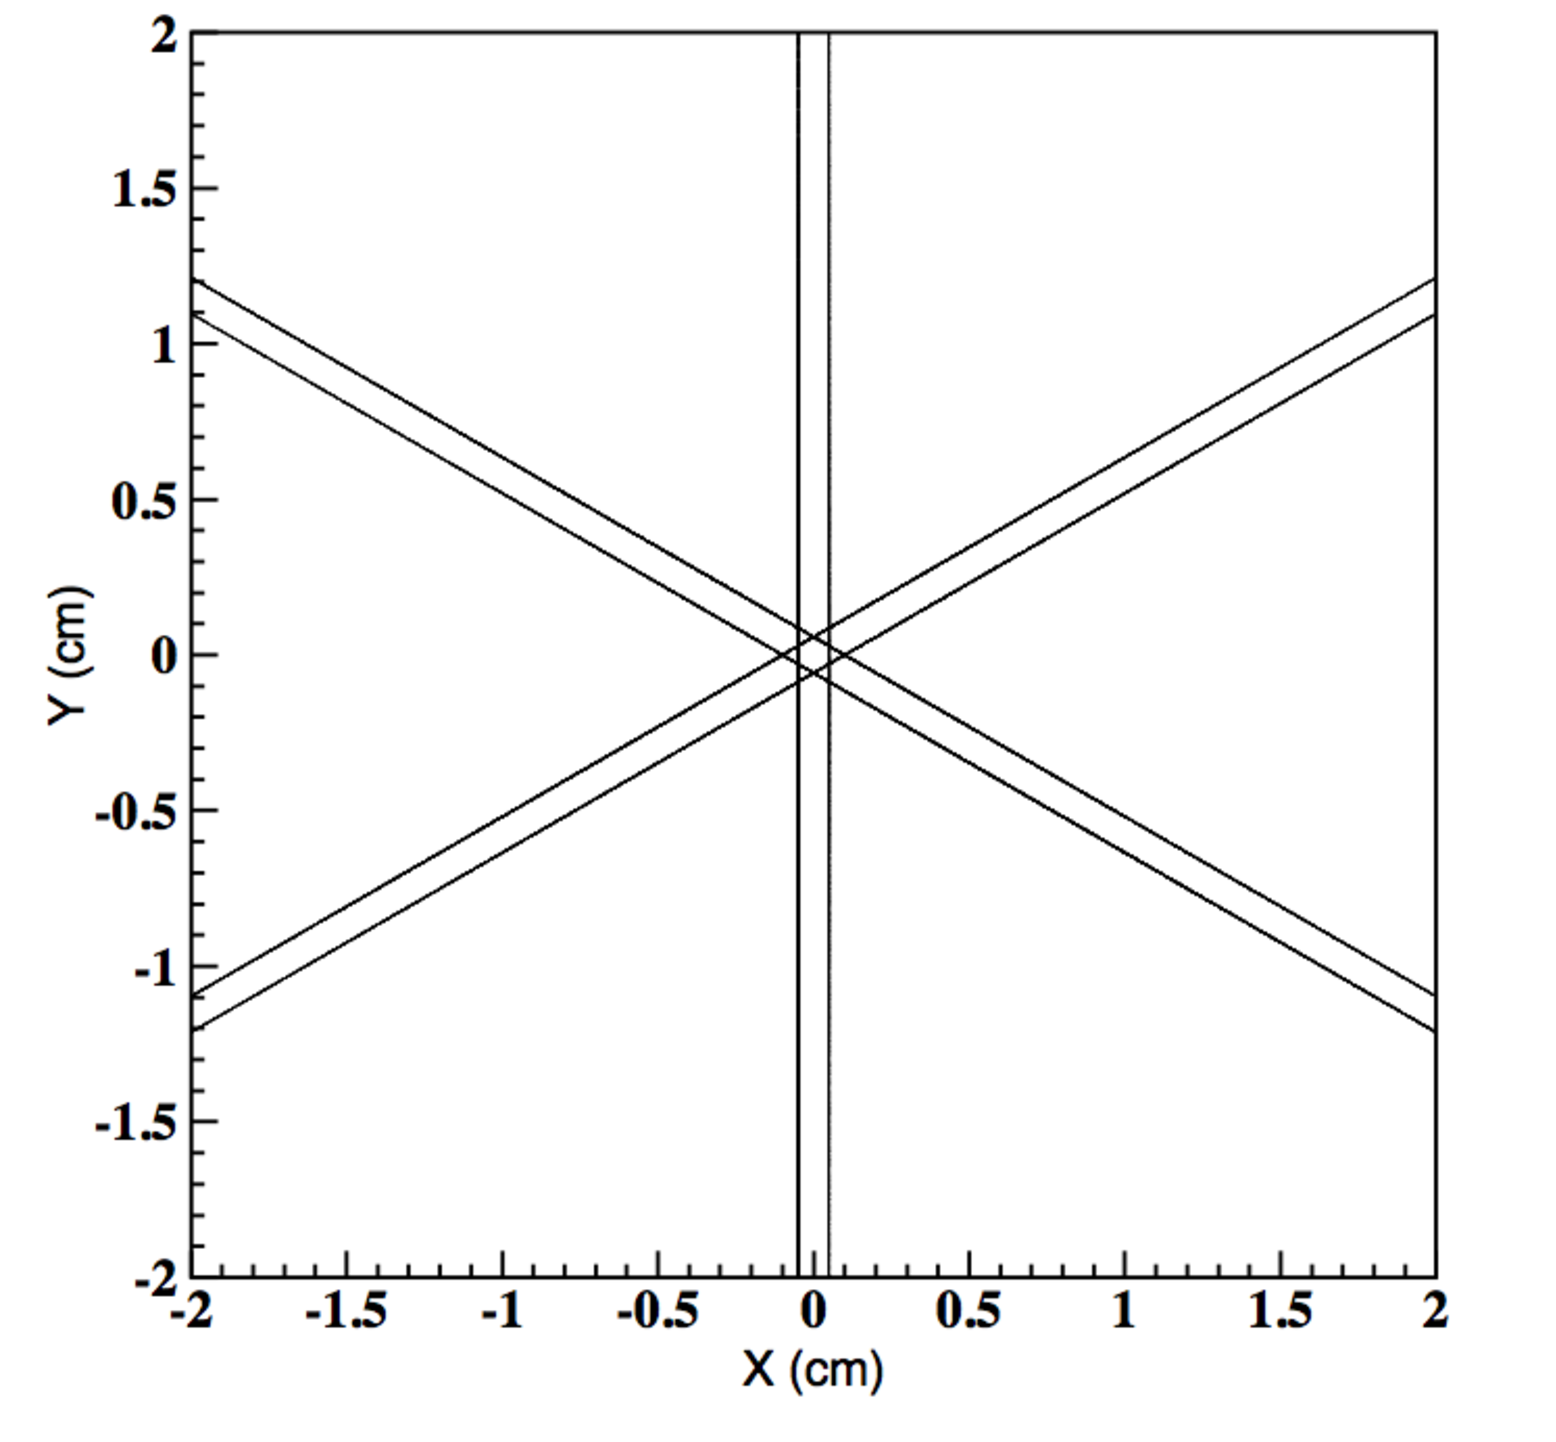
\includegraphics[width=0.75\textwidth]{track_xy_close}
\caption{Vertex ($XY$) coordinate for charged tracks in CLAS, closer look.}
\label{fig:xytrackc}
\end{center}
\end{figure}

\section{CLAS/eg6}

CLAS eg6 experiment used solenoid setup and therefore correct vertex reconstruction is important for correct determination of the CLAS track parameters at the true vertex. In addition to CLAS, eg6 run used a Radial Time Projection Chamber (RTPC) located around the target, inside the solenoid field (target was symmetrically position inside the solenoid field in Z-direction). Tracks in RTPC were fitted using the beamline as a constraint, and therefore the correct beam position is important for RTPC track fitting as well. 

Studies have been conducted to determine the true beam position on ($XY$) plane in the CLAS coordinate system for eg6. Eg6 target was a $30$ cm long $6$ mm ID kapton tube with $6$ atm pressurized $^4$He gas. It has two aluminum windows of $15$ $\mu m$ thick from the upstream and downstream ends. Particle reconstruction in CLAS from the upstream window was somewhat skewed by massive upstream support, that served also as a gas inlet-outlet port for the target. The downstream one had a clear site to the CLAS detector region and hanse particles were reconstructed more cleanly. Downstream window position as a function of azimuthal angle of tracks in CLAS has been used to define beam ($XY$) position. 

\subsection{Eg6 6 GeV run}

In top graph of Fig.\ref{fig:phiz} Z-vertex distribution of electrons detected in polar angular range from $\theta=29^\circ$ to $\theta =31^\circ$ vs. electron azimuthal angle is presented. Both windows of the target cell are visible. The upstream window looks fuzzy, while downstream window is sharp, well defined vertex. The closer look to the downstream end of the target is shown in bottom graph of Fig.\ref{fig:phiz}. Azimuthal ($\phi$) angle dependence is clearly seen. This dependence indicates that the beam direction is shifted from $X=0$ and $Y=0$ point in CLAS coordinate system.    

\begin{figure}[htb]
\begin{center}
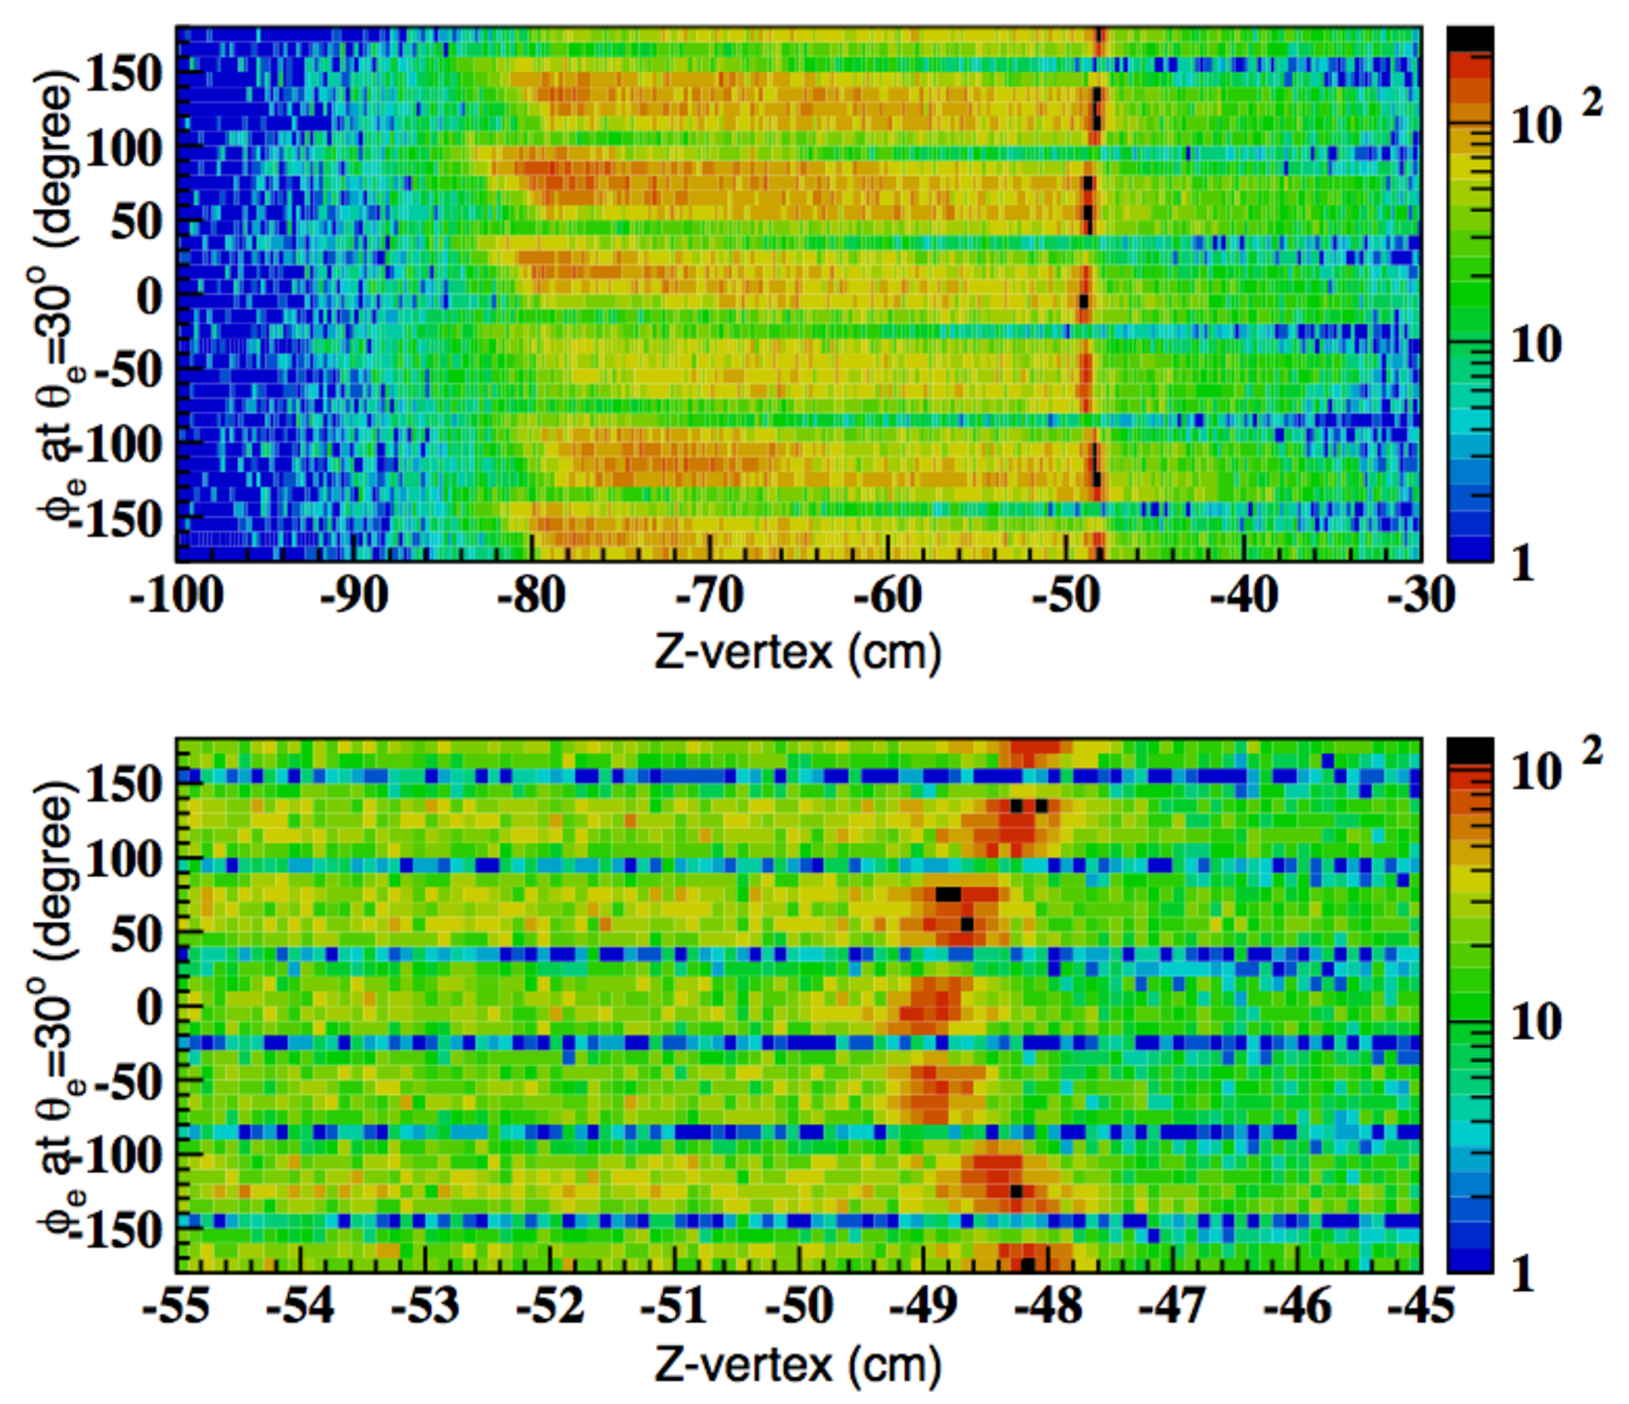
\includegraphics[width=0.9\textwidth]{phi_z_eg6.pdf}
\caption{Z-vertex versus azimuthal angle of electrons measured in CLAS in the polar angular range $29^o$ to $31^o$.}
\label{fig:phiz}
\end{center}
\end{figure}

Schematically Z-vertex displacement for tracks at $\phi=\phi_0$ and $\phi=\phi_0+\pi$, when beam position on ($XY$) plane is ($x_by_b$),  is shown in Fig.\ref{fig:phid}. Here $\phi_0=\tan({y_b/x_b})$. The way tracking reconstructs the vertex, tracks at $\phi_0$ will have Z-vertex reconstructed upstream of true vertex ($Z_R$), while tracks at $\phi=\phi_0+\pi$ will have Z-vertex downstream of the true vertex ($Z_L$).  The azimuthal ($\phi$) dependence of the Z-vertex will be given by:
\begin{equation}
Z=a-b*\cos(\phi-\phi_0)/\tan\theta
\label{zfun}
\end{equation}
where $a=Z_0$ is the true vertex, $b$ is the distance of the beam position from $X=0$, $Y=0$ point, $b=\sqrt{x_b^2+y_b^2}$, and $\theta$ is the polar angle of the track.

\begin{figure}[htb]
\begin{center}
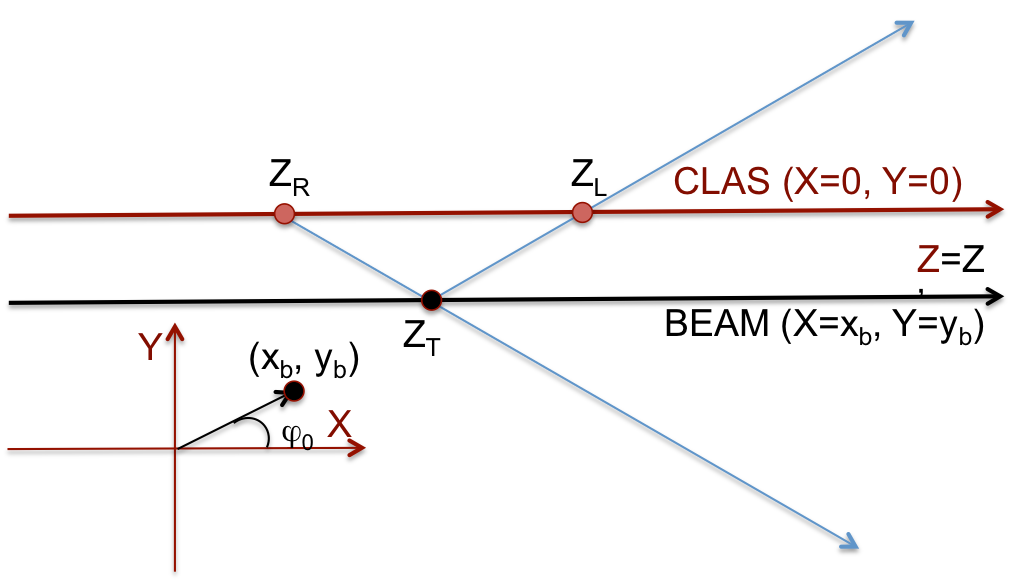
\includegraphics[width=.67\textwidth]{vertex_displacement.pdf}
\caption{Schematic description of the vertex displacement due to beam position offset in ($XY$) plane.}
\label{fig:phid}
\end{center}
\end{figure}

Using electrons scattered at $\theta\approx30^\circ$ (from $29^\circ$ to $31^\circ$) from the downstream window of the target parameters $a$, $b$ and $\phi_0$ were found for eg6 $6$ GeV runs. In Fig.\ref{fig:ze2931} dependence of the reconstructed $Z$ position of the fitted peak corresponding to the downstream window is shown (points). Curve corresponds to the fit using formula in Eq.(\ref{zfun}). From the fit $\phi_0=-189.6^\circ$, $a=-48.52$ cm, and $b=0.24$ cm. Using $\phi_0$ and $b$ one can calculate $x_b=-b\times \cos(\phi_0)=0.237$ cm and $y_b=-b\times\sin(\phi_0)=-0.04$ cm.  This coordinates must be taken into account when tracks are extrapolated to the production vertex. There are two ways of doing it, first one is by fixing the CLAS tracking algorithm to find DOCA of the track and the beam direction, second is to introduce ad hoc corrections to fix the vertex parameters. The second method is easier, especially for such a small displacement (eg1 experiment had such corrections over larger radius due to the rastered beam).  

\begin{figure}[htb]
\begin{center}
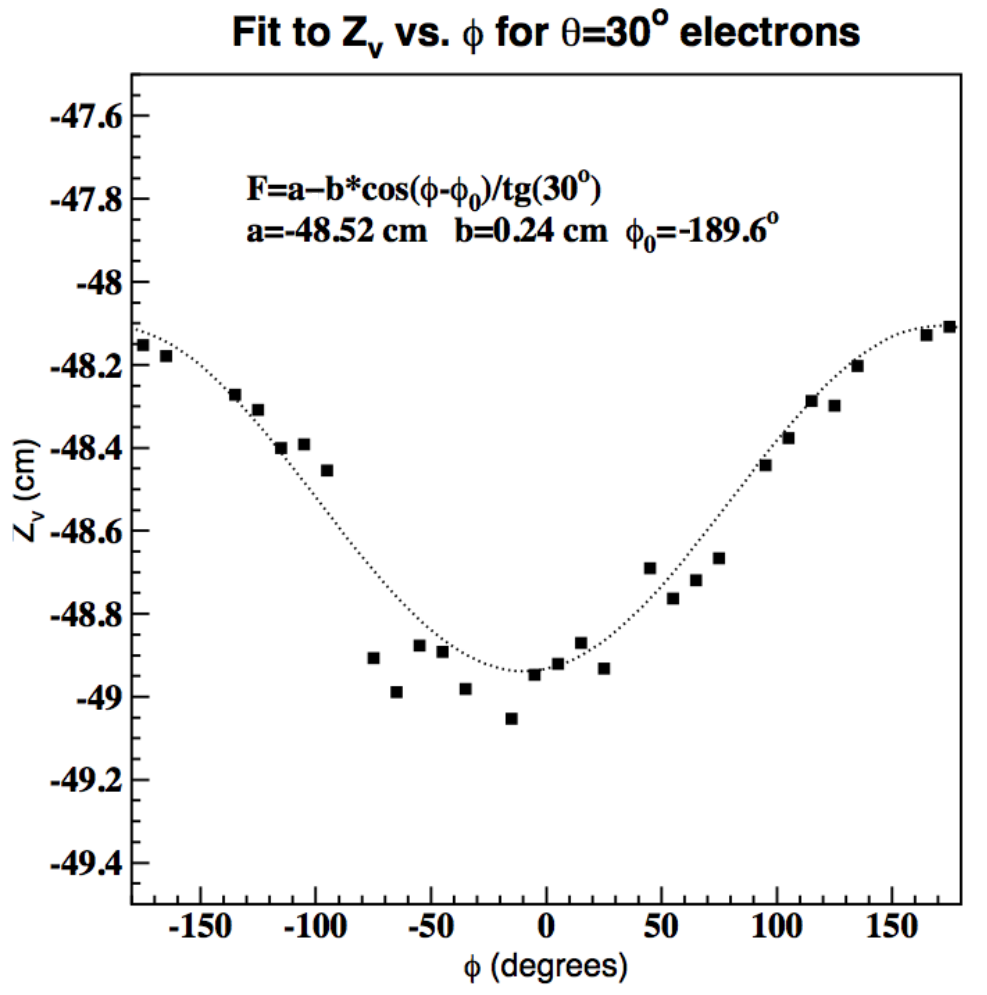
\includegraphics[width=.7\textwidth]{beam_xy_fix.png}
\caption{Fit to Z-vertex of electrons scattered from the downstream window of the target in the polar angular range $29^o$ to $31^o$ for 6 GeV data.}
\label{fig:ze2931}
\end{center}
\end{figure}

\clearpage

\subsection{Eg6 1.2 GeV run}

The same study was also performed for EG6's 1.206 GeV data used to calibrate the RTPC and is shown in the Fig.~\ref{fig:zphi1gev}.  In this case, the result was a beam offset of $x=1.55$ mm and $y=0.29$ mm.  

\begin{figure}[htb]
\begin{center}
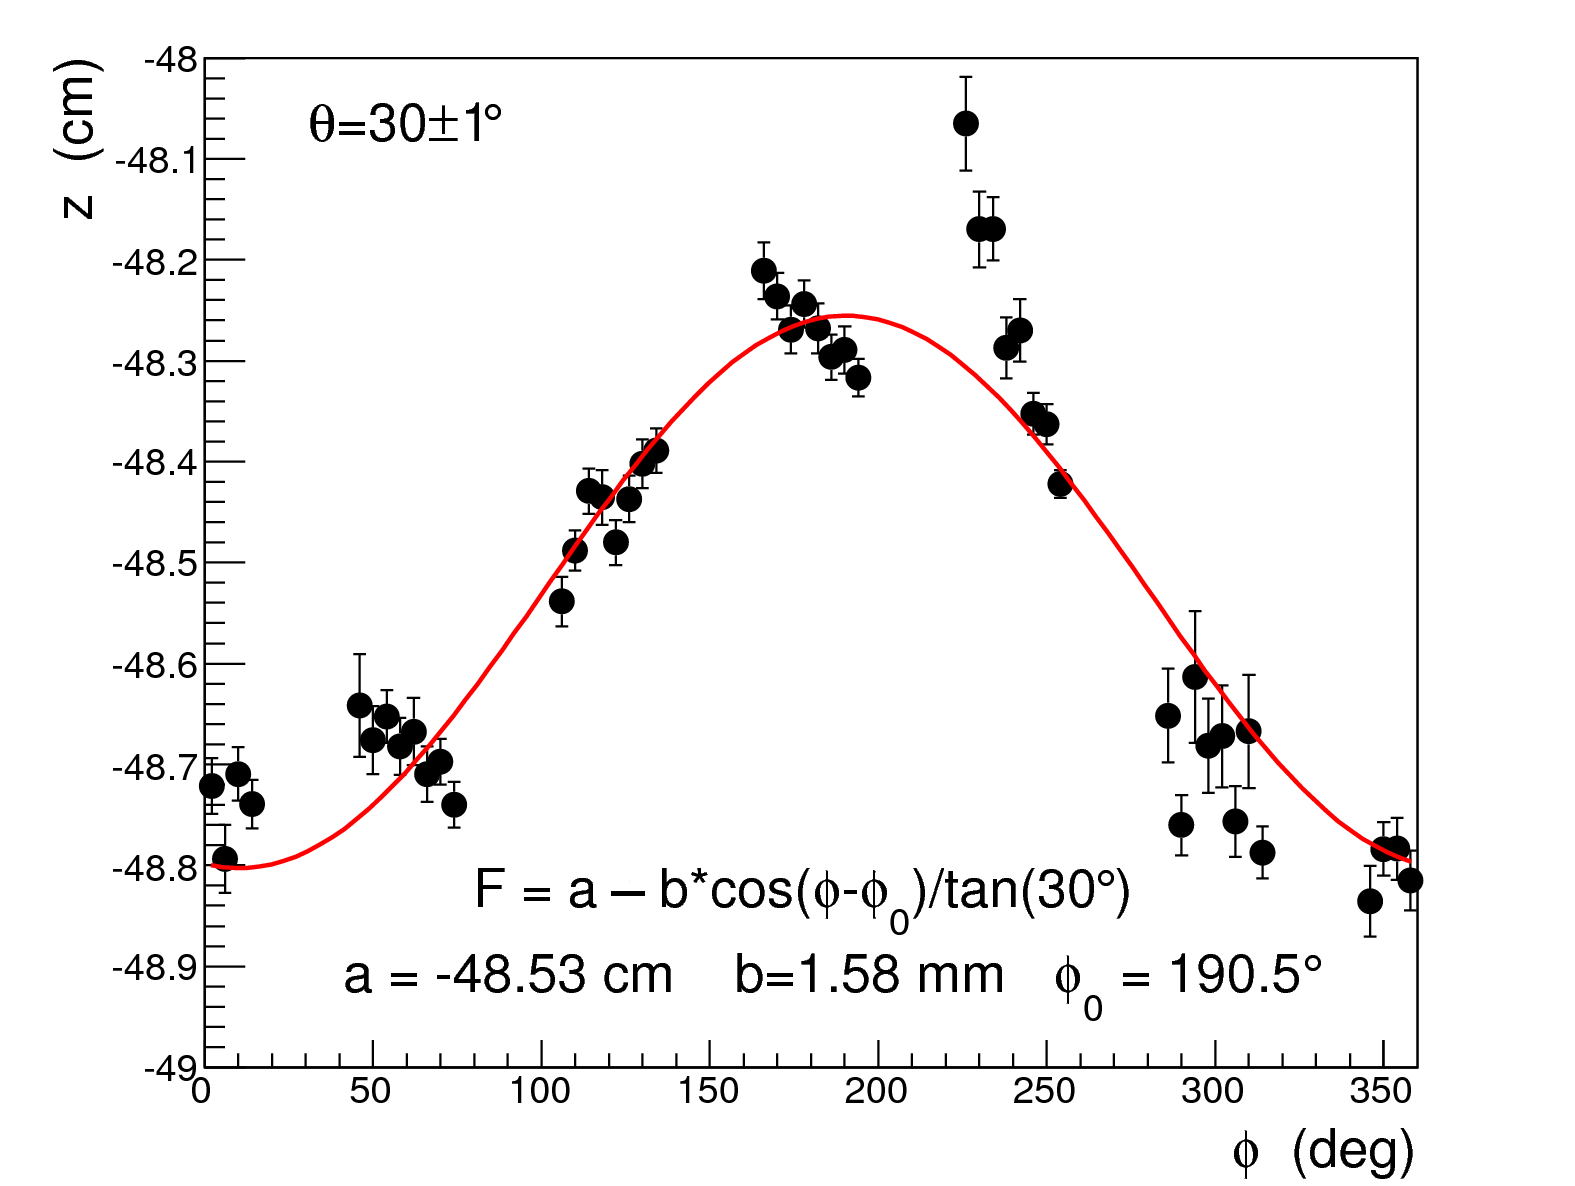
\includegraphics[width=0.85\textwidth]{zphi_1gev_fix.png}
%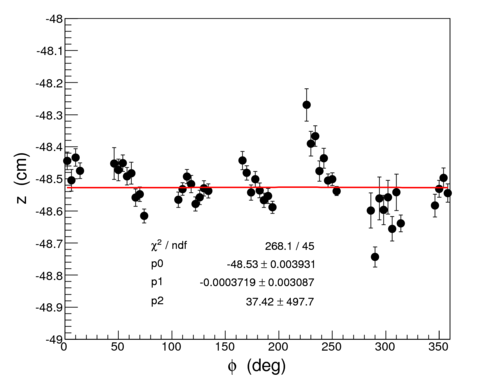
\includegraphics[width=0.495\textwidth]{zphicorr_1gev.png}
\caption{Fit to Z-vertex of electrons scattered from the downstream window of the target in the polar angular range $29^o$ to $31^o$ for 1.206 GeV data.
\label{fig:zphi1gev}}
\end{center}
\end{figure}

\noindent

Studies are ongoing to use the corrected electron vertex as a reference to compare with the recoil vertex to measure the misalignment of the RTPC.



%Figure \ref{fig:zrtpc_clascorr} shows the results of fitting $\delta z$ as a function of $\phi_{RTPC}$.  The result is an offset of $(x,y)=(2.8,-1.33)$.  Attributing this offset to RTPC misalignment instead of beam offset, which is already corrected, the conclusion is an RTPC misalignment of $(-2.8,1.33)$ relative to the beamline.

%The result is an RTPC misalignment $(x,y)$ relative to the beamline of (-2.5,1.0) and  an RTPC misalignment relative to (0,0) of about (-4,1).  Units are millimeter.

%\begin{figure}[htb]
%\begin{center}
%\includegraphics[width=0.8\textwidth]{zrtpc_clascor.png}
%\caption{Fit to difference between Z-vertex of electrons in CLAS and recoils in RTPC.  Recoil polar angle is limited to $60^o\pm5^o$ in RTPC.  }
%\label{fig:zrtpc_clascorr}
%\end{center}
%\end{figure}

\section{Ad Hoc corrections}


Correction of the Z-vertex coordinate is simple, just reversing functions in Eq:(\ref{zfun}).  Corrected vertex then will be:
\begin{equation}
Z_{corr}=Z+b\times\cos(\phi-\phi_0)/\tan\theta
\label{eq:zcor}
\end{equation}

In Table~\ref{tab:param}, parameters of the fit to the downstream window using Eq.(\ref{zfun}) for both energy settings are presented. In Fig. (\ref{fig:ezcor}) corrected $Z$-vertex of electrons in $6.064$ GeV runs is shown. As expected the distribution on the right does not show any $\phi$ dependence. Fit to the projection of the downstream window position on the z-axis resulted to $\sigma=4.3$ mm vertex resolution. Corrected vertex distributions for negatively and positively charged hadrons are shown in Fig. \ref{fig:zcor_pn}. No dependence on azimuthal angle after applying correction of Eq.(\ref{eq:zcor}).
The result of using the vertex correction for $1.2$ GeV data is shown in Fig.~\ref{fig:zphi1gev_corr}, and the $\phi$ modulation is removed as expected.

\begin{table}[htdp]
\caption{Parameters of fits to Z-vertex dependence on $\phi$ for eg6 data sets.}
\begin{center}
\begin{tabular}{|c|c|c|}
\hline
Parameter& E$_{beam}=6.064$ GeV & E$_{beam}=1.206$ GeV  \\
\hline
$Z_0$ &$-48.52$ cm& $-48.53$ cm \\
$b$ & $2.4$ mm& $1.58$ mm \\
$\phi_0$& $-186.6^\circ$&$190.5^\circ$ \\ \hline
$x_b$  & $2.37$ mm & $1.55$ mm \\
$y_b$  & $-0.4$ mm & $0.29$ mm \\
\hline
\end{tabular}
\end{center}
\label{tab:param}
\end{table}%

\begin{figure}[htbp]
\begin{center}
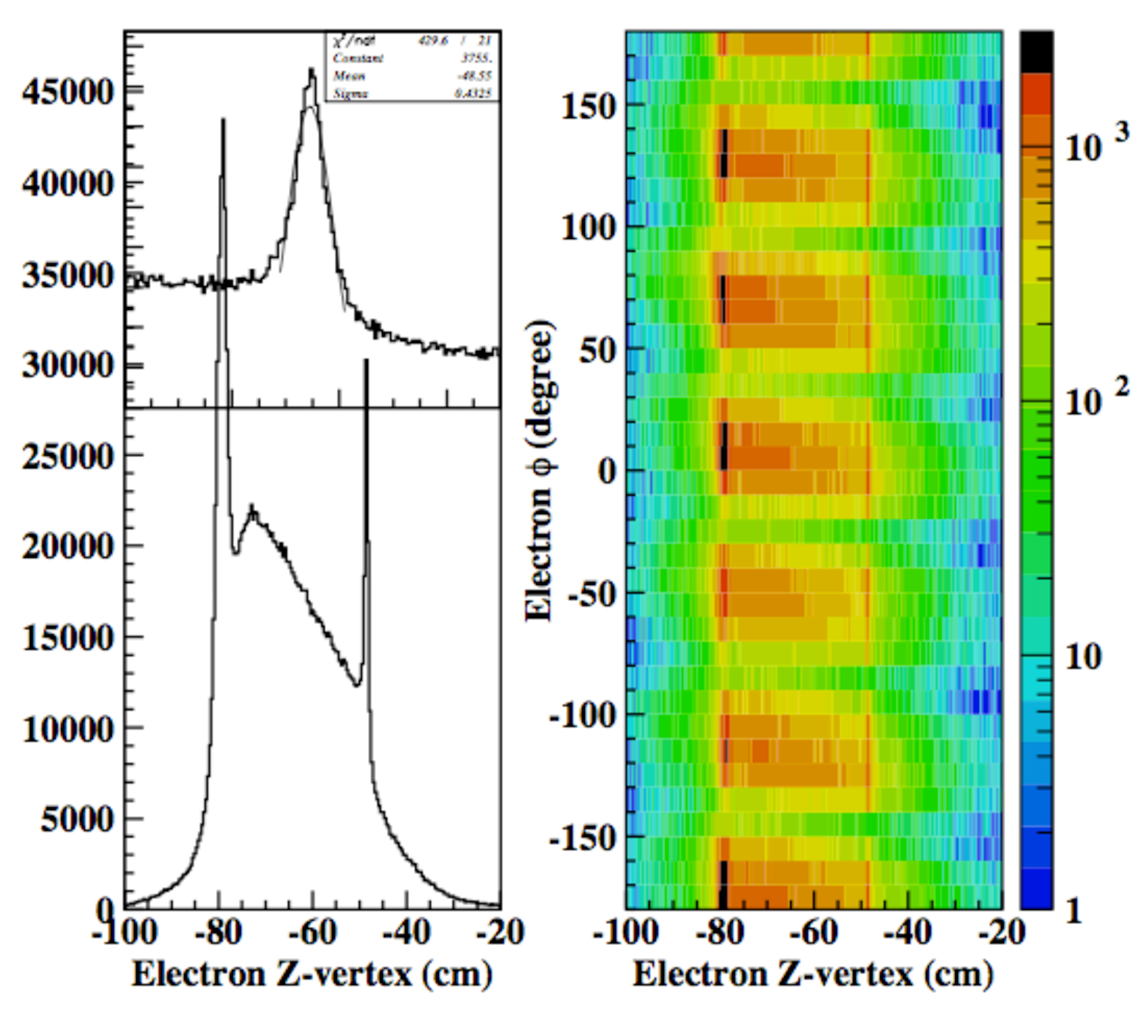
\includegraphics[width=.8\textwidth]{zelectron_corrected}
\caption{$\phi$-dependence of corrected Z-vertex for electrons using Eq.(\ref{eq:zcor})}
\label{fig:ezcor}
\end{center}
\end{figure}

\begin{figure}[htbp]
\begin{center}
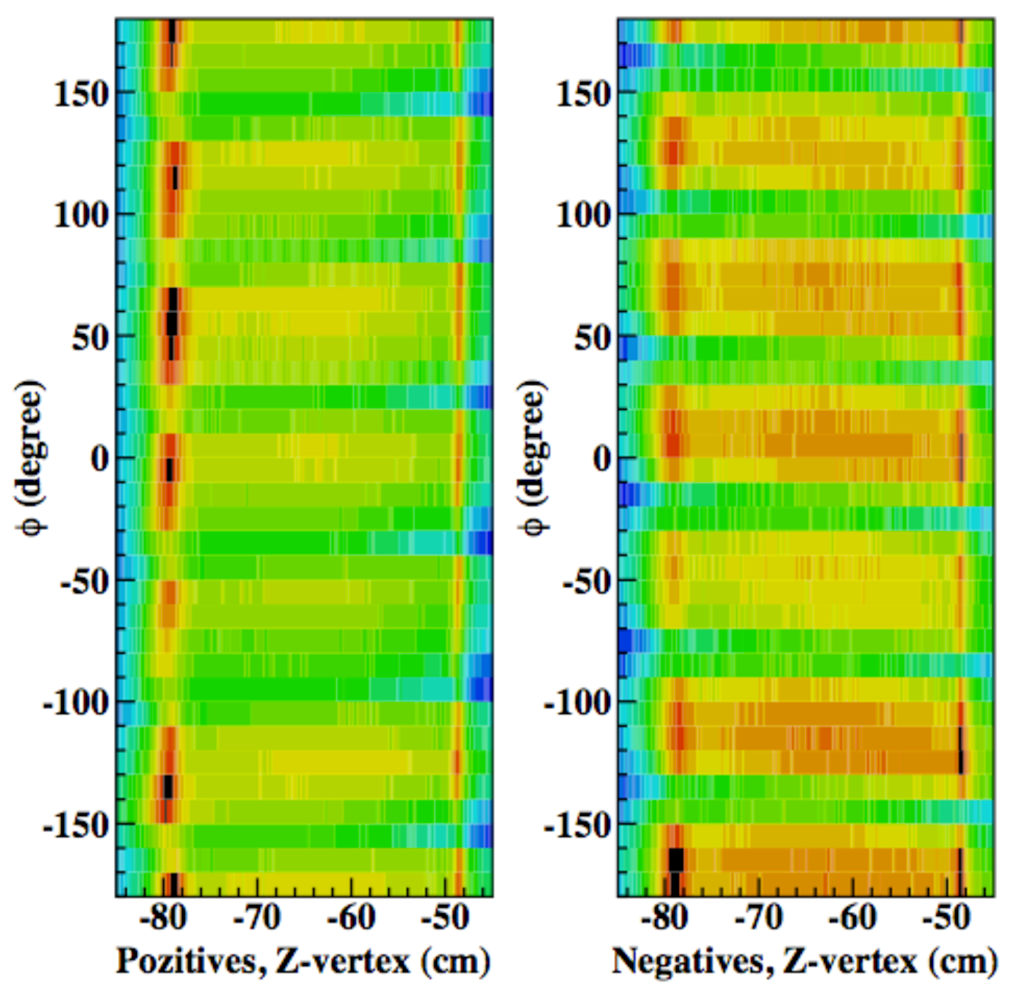
\includegraphics[width=.8\textwidth]{pos_neg_zvert}
\caption{$\phi$-dependence of corrected Z-vertex for positively (left) and negatively (right) charged hadrons using Eq.(\ref{eq:zcor})}
\label{fig:zcor_pn}
\end{center}
\end{figure}



\begin{figure}[htb]
\begin{center}
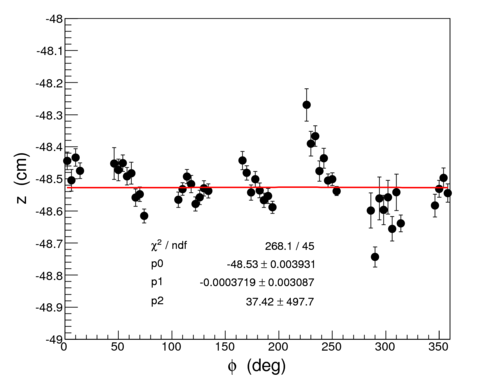
\includegraphics[width=0.8\textwidth]{zphicorr_1gev.png}
\caption{Same as Fig.~\ref{fig:zphi1gev} but after the correction of Eq.\ref{eq:zcor}.  The $\phi$-modulation is removed as expected.
\label{fig:zphi1gev_corr}}
\end{center}
\end{figure}

\end{document}
